% Chapter Template

\chapter{FM-Index} % Main chapter title

\label{Chapter2} % Change X to a consecutive number; for referencing this chapter elsewhere, use \ref{ChapterX}

%----------------------------------------------------------------------------------------
%	SECTION 1
%----------------------------------------------------------------------------------------
%\begin{figure*}[h]

%	\vspace*{-60mm}
%	\hspace*{60mm}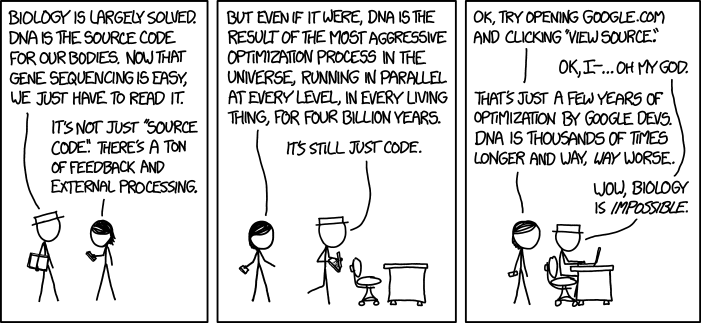
\includegraphics[scale = 0.3]{Figures/xkcd.png}
%\end{figure*}
%\vspace*{15mm}

With the observations foretasted about the nature and form of the data in the context of genomics, it seems obvious that an appropriate data structure for those, along with an efficient algorithm, might to a serious gain in performance in the short reads alignments. The \textsl{FM-Index} is a lossless compression algorithm based on the \textsl{Burrows-Wheeler Transform} that offers such gains by reorganizing the data in a way that may reduce both memory needs and latency of the mapping process. 

Both those concepts are the subject of the next sections, followed by a \textsl{Python} implementation, which aims to better illustrate the whole read alignment process, and a \textsl{C++} implementation of the same algorithm which will be then used for the hardware implementation.

\section{Theoretical Concepts}

Introduced by \textsl{Michael Burrows} and \textsl{David Wheeler} in 1994, the \textsl{Burrows-Wheeler Transform} (BWT) rearranges the characters of a \textit{string} into sequences of similar characters by a sequence of linear operations. Although it does not reduce the size of the input data, the rearrangement thus obtained gets greatly improved compression results. Furthermore, the easy reversibility of the process substantially facilitate data manipulation employed in sequence alignment, such as finding the original position from the determined one in the transform. This process is further detailed in the next section.

\subsection{Burrows-Wheeler Transform Algorithm \& LF-Mapping}

The transform can be divided in 4 main steps \footnote{BWT0} :
\begin{enumerate}
\item Append a special character (usually represented as a \$), lexicographically smaller than any others, at the end of the input string \textrm{T}.
\item Construct a square matrix $M_T$ with each being another iteration of a left rotating shift applied to the original string.
\item Sort $M_T$ in lexicographical order
\item Get the transformed text output $T^{bwt}$ by selecting the last column of $M_T$ 
\end{enumerate}

\begin{figure}[h]
\centering
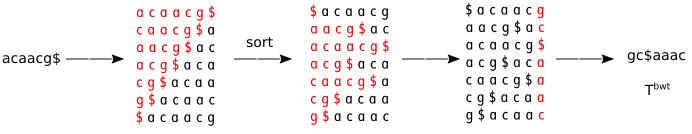
\includegraphics[scale=0.65]{Figures/bwt.png}
\caption{Illustration of the \textsl{BWT} applied to the string \textit{acaacg}}
 \label{fig:bwt}
 \end{figure}
The figure \ref{fig:bwt} above illustrates the process of the \textsl{BWT}, it will be shown next what is used in the mapping process, but first let us note the following properties :
\begin{enumerate}
\item the process is revertible as it consists exclusively of linear operations
\item all columns are permutations of the input $T$
\item the last columns contains mostly all similar character consecutively
\item the first column contains all characters in lexicographical order, so the first row will always start with the inserted \$ symbol (i. e. be the first rotation applied to $T$)
\item Occurrences of a character $c$ in the first column are sorted the same way than in the last column, meaning ranks order in the first and last column match, as depicted in figure \ref{fig:LF}
\end{enumerate}



From a compression perspective, the $T^{bwt}$ result is a way better candidate than its original form as it sees most of similar characters regrouped, hence allowing shorter encoding for those sequences\footnote{http://www.hpl.hp.com/techreports/Compaq-DEC/SRC-RR-124.pdf}. Furthermore, properties 1, 2 and 5 indicate an easy transition, if needed, back to the original text  using the  \textsl{LF Mapping} illustrated in figure \ref{fig:LF} and formally defined in equation \ref{eq:LF}. \\

For $Occ$ an array containing, for each symbol $c$ of the alphabet $\Sigma$, the index of its first occurence in the first column $F$ and $Count(i, c)$, a function returning the number of occurences of $c$ in $F$ at given index $i$, we can define the $LastToFirst$ mapping as follow :
\begin{equation}
    LF(i, c) = Occ[c] + Count(i, c)
    \label{eq:LF}
\end{equation}


\begin{minipage}[t]{0.5\textwidth}
    \begin{figure}[H]
\hspace{-15mm}  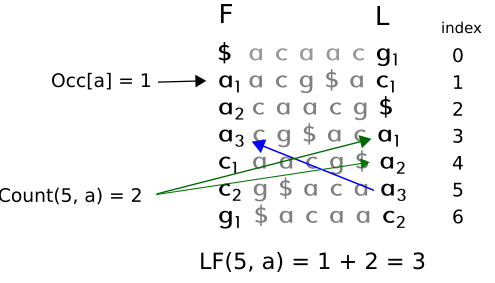
\includegraphics[scale = 0.45]{Figures/LF.png}
  \caption{LF-Mapping of $3^{rd}$ occurrence of $a$ }
    \label{fig:LF}
\end{figure}
\end{minipage}
\begin{minipage}[t]{0.45\textwidth}
        This figure illustrates how the mapping is done : from the fact that character ranking are the same in both last and first column (and all the others for that matter), the \textsl{LF-Mapping} algorithm enables retrieval of the position in $F$ for any character in $L$. This method is used in the \textsl{Walk-Left} algorithm to reconstruct the original text, which is thereafter further detailed in figure \ref{fig:walkleft}.
\end{minipage}
\vspace*{5mm}

Finally, from a search point of view, the last property is the most interesting. Lexicographical order allows for spatial proximity of sought result, hence, an iterative search through a word to find in $T^{bwt}$ will see each iteration to indicate spatially close positions which yet facilitates this process.\\

Now that this concept is well defined, the next section will aim to illustrate how the FM-Index algorithm makes the best out of this transform in order to enable efficient data compression and sub-string queries.

\subsection{FM-Index}

An \textsl{FM-Index} is a lossless text compression based on the \textsl{BWT}\footcite{FM\_INDEX}, it was created by \textsl{Paolo Ferragina} and \textsl{Giovanni Manzini} whom refer to it as an \textit{"opportunistic data structure"}. The design of this index is based upon the combination of the BWT and the suffix array data structure, displayed in red in figure \ref{fig:bwt}.\footnote{https://pdfs.semanticscholar.org/d896/e62b6cbfd623d1d9041f90b7f9e41d1451a7.pdf}

\paragraph{Creating an FM-Index}

In order to create the \textsl{FM-Index} of an input full-text \textit{string} $T$, one must create its \textsl{BWT} transform $T^{bwt}$ as explained in the previous section. Referring again to figure \ref{fig:bwt}, the \textcolor{red}{red} sub-matrix from the one in the middle, i.e. the suffix array (SA) will also be used. Finally, the index itself, noted $F$ will be constructed from the SA and $T^{bwt}$. \\

For a given $T^{bwt}$ of $N$ symbols on an alphabet $\Sigma$ of $\sigma$ elements, we define the FM-Index $F$ as a two-dimensional matrix with $(N + 1)$ rows and $\sigma$ column. Hence, the entry at index $i$ (row) and for symbol $c$ (column), $F[i][c]$ contains the number of occurrences of $c$ before the index $i$ in $T^{BWT}$. From this definition, we can construct the whole index for $T^{bwt}$, initializing $F[0]$ at $0$ and $\forall$ $i$ from $0$ to $N$, copy $F[i]$ into $F[i+1]$, incrementing $F[i+1][c]$ only if $T^{BWT}[i]$ = $c$. The last entry $F[N + 1]$ represents the total number of occurrences of all symbols in $T^{bwt}$. This whole structure of the FM-Index is given an example in the figure \ref{fig:fmindex} below. \\

\begin{minipage}{0.5\textwidth}
\begin{figure}[H]
    \hspace{-15mm}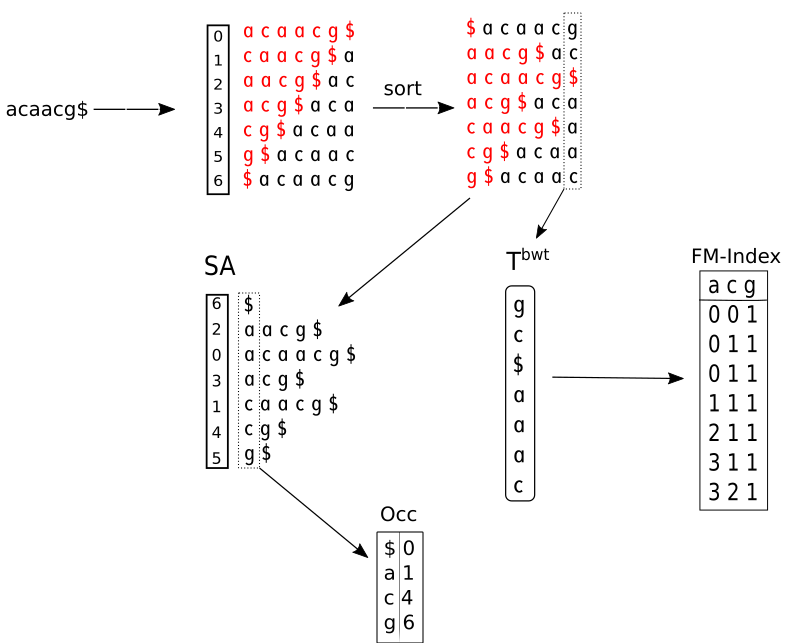
\includegraphics[scale = 0.35]{Figures/FMIndex.png}
    \caption{Illustration of the FM-Index construction from "$acaacg$"}
    \label{fig:fmindex}
\end{figure}
\end{minipage}
\hspace{15mm}
\begin{minipage}{0.3\textwidth}
After applying the BWT to the input text, the suffix array is extracted and from it, the $Occ$ array. From the transform itself, the FM-Index $F$ is filled. \\
Note that in this case, $F$ replaces the function $Count$ described in the previous section in this schema as it is directly read by it.
\end{minipage}


\paragraph{String Matching and Walk-Left Algorithms} To now implement the string search using the FM-Index, two algorithms are used. The first, initially used to fully revert the BWT, can be exploited to determine the position of a string in the original text from its position in the suffix array. This position can be determined using the second algorithm, Walk-Left, which, given a string $q$ scans the suffix array using LF-Mapping, in order to determine a position range in which $q$ is located. Note that this interval might be empty, in which case $T$ does not contain $q$ or of length $\geq$ 1, in which case its length corresponds to the number of occurences of $q$ in $T$. \\
Those algorithms are described in \ref{alg:WL} and \ref{alg:match} and a graphical example of execution are provided by Figures \ref{fig:walkleft} and \ref{fig:match}.

\begin{figure}[H]
    \centering
    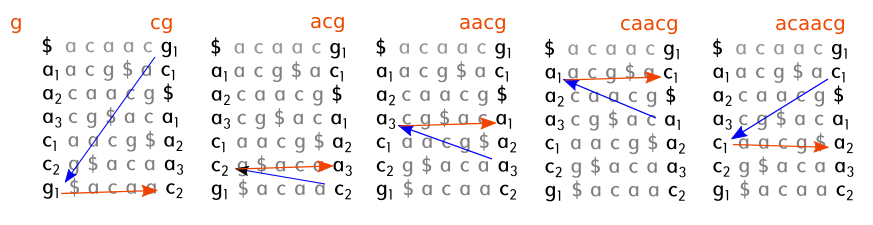
\includegraphics[scale=0.5]{Figures/WL.png}
    \caption{Illustration of the BWT inversion using Walk-Left\cite{genomic}}
    \label{fig:walkleft}
\end{figure}

\begin{minipage}[t]{0.45\textwidth}
\begin{algorithm}[H]
	\SetAlgoLined
	\KwIn{BWT $T^{bwt}$, FM-Index $F$, First occurrences $Occ$}
	\KwOut{The original input string $T$}
	i = 0\;
	t = ""\;
	\While{$T^{bwt}[i] \neq $ "\$"}{
		t = $T^{BWT}[i] $ + t\;
		i = $LF(i, T^{BWT}[i])$\;
	}
\caption{Walk-Left - Inverting the BWT}
\label{alg:WL}
\end{algorithm}
\end{minipage}
\begin{minipage}[t]{0.45\textwidth}
\begin{algorithm}[H]
\SetAlgoLined
\KwIn{BWT $T^{bwt}$, FM-Index $F$, $Occ$, query string $q$}
\KwOut{Range $top$, $bot$ for $q$ in suffix array}
	$top$ = 0\
	$bot$ = $len(T^{BWT})$\;
	\For{$qc$ in $reverse(q)$}{
		$top$ = $LF(top, qc)$\;
		$bot$ = $LF(bot, qc)$\;
}
\caption{Exact String Matching in SA}
\label{alg:match}
\end{algorithm}
\end{minipage}

\vspace*{5mm}


\paragraph{Putting it all Together}

Now that all the data structures and computational tools have been introduced, we can define the process of exact string matching using the FM-Index, in an input reference string $T$ and a string query $q$ :
\begin{enumerate}
\item Compute the Burrows-Wheeler Transform $T^{bwt}$ of $T$, use it to find $Occ$ and to get the FM-Index $F$.
\item Use Algorithm 2 to determine the index of the rotation in the implicit suffix array containing $q$
\item If such an index exists (i.e. $q$ occurs at least once in $T$), use the Walk-Left Algorithm to walk back to the beginning of the text from this index i.e. until the algorithm reaches the \$ character.
\item The number of steps it takes to do so corresponds to the offset of $q$ in $T$
\end{enumerate}

\begin{figure}[H]
    \centering
    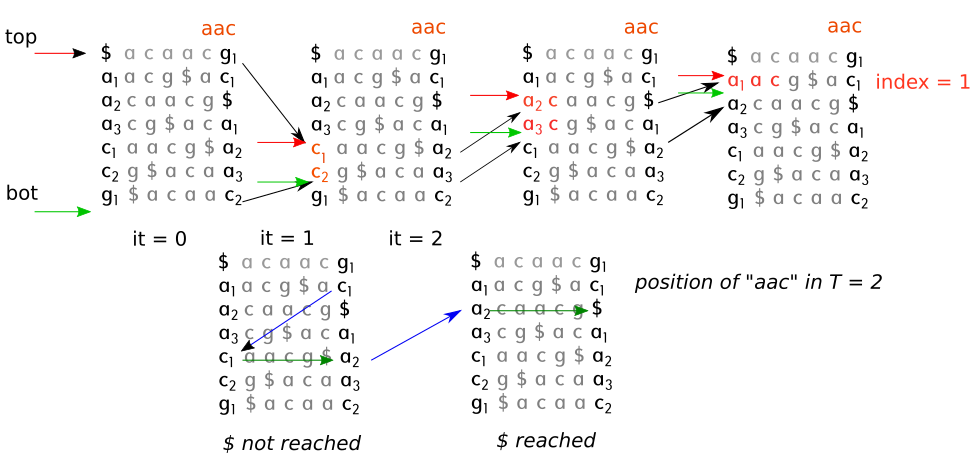
\includegraphics[scale=0.4]{Figures/MATCH.png}
    \caption{Finding position of $aac$ in example $T$ \cite{genomic}}
    \label{fig:match}
\end{figure}

\paragraph{Optimization Benefits of the FM-Index over BWT}

As mentioned earlier in this document, the size of a genomic dataset is usually in the billion of entry range. Hence, the structures showed in Figures \ref{fig:fmindex}, if used fully as displayed, may pose some issues. First, the number of step it might require \textsl{Walk-Left} to reach the beginning of $T$ is linear to the length of said $T$, thus implying potentially billions of iterations if the FM-Index $F$ is not used. Furthermore, storing the whole suffix array, along with the whole FM-Index for the \textsl{LF-Mapping} function requires two arrays, both with a number of row corresponding to the length $N$ of $T$ and a various number of columns. Even with a reduced alphabet size, storing those two structures would require an enormous amount of memory. \\

From those observations, some optimization trade-off are made,  finding a middle ground between time performances and memory requirements :
	\begin{itemize}
		\item [-] In order to speed the \textsl{Walk-Left} algorithm up, an idea would be to store the post-sorting suffix array indices, as shown in Figure \ref{fig:fmindex}. For a given position in the sorted suffix array, this index would indeed be the direct value of the position of the queried string in the original text. However, keeping in mind that memory is in this context a very valuable resources, storing all those values does not seem like a workable idea. An acceptable compromise would be to only keep samples \footnote{MIT} of this array (e.g. one entry every $32^{th}$ rows). Using this, the \textsl{Walk-Left} algorithm would "walk", until it comes across a sampled row. It would then suffice to add the number of steps it took to get to this position, added to the store sample, to obtain the desired position in the original text. This idea is illustrated in Figures \ref{fig:opti}.

		\item [-] Along the same lines, instead of storing the whole \textsl{FM-Index} $F$, keep only some samples (e.g. one every 128 entries), which are later referred to as \textit{checkpoints}. For a given index $i$, if no checkpoints is available, read up or read down (depending on the closest checkpoint location), counting the occurrences of the symbol at $i$ along the way to add or subtract this count to the value eventually found.
				\end{itemize}
	
Both those modifications, although coming from opposite situations, meet in the same trade-off : offering constant time computation while limiting the amount of required space to store those structures. An example of those modifications is presented in Figures \ref{fig:checkpoints} and \ref{fig:ssa}.


		\begin{figure}[h]
			\centering
			\begin{subfigure}{.5\textwidth}
				\centering
				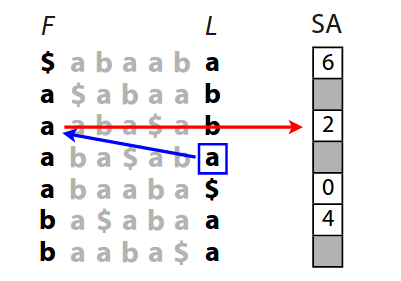
\includegraphics[width=.5\linewidth]{Figures/sa.png}
				\caption{TODO SA sample example}
				\label{fig:ssa}
				\end{subfigure}%
				\begin{subfigure}{.5\textwidth}
					\centering
					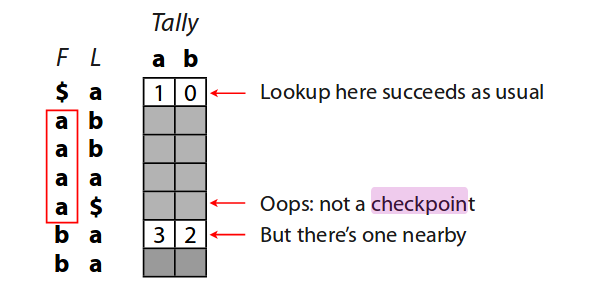
\includegraphics[width=.8\linewidth]{Figures/CHECKPOINT.png}
					\caption{TODO Checkpoint example}
					\label{fig:sub2}
					\end{subfigure}
					\caption{Illustration of the two proposed improvement}
					\label{fig:checkpoints}
					\end{figure}


\section{C++ Implementation}

All the software components of this project interacting with the board will be written in \textsl{C++}. This choice is based on the performance oriented aspect of this project, along with the need to precisely define binary data structures and the use of a pre-existing API implementing a communication interface with the used board, the \textit{Pico API}, further detailed in the next chapter. The need for precise and custom data structures comes from the need to define a precise encoding of the \textsl{nucleotide reads} to be used on the FPGA system along with well defined and space-optimized data structures to store the \textsl{BWT} in the memory, the suffix array samples and the FM-Index checkpoints. Those elements are showed in the next section, followed by an operating diagram and an example of execution.

\subsection{Reads encoding and Data Structures}

\paragraph{Reads encoding}

Considering there are 4 different nucleotides within any DNA sequence, adding the uncalled base N type read and the "\$" equivalent character, we need to encode 6 symbols and thus need at least 3 bits. Therefore, it has been chose to use the following encoding : \\

\begin{minipage}[c]{0.35\textwidth}
\vspace*{6mm}
	\begin{tabular}{|c|l|}
	\hline
		Name & Encoding \\
		\hline 
		"\$" & 001 \\
		A & 010 \\
		C & 011 \\
		G & 100 \\
		N & 101 \\
		T & 110 \\
    \hline
	\end{tabular}
\end{minipage}
\begin{minipage}[t]{0.85\textwidth}
\vspace*{-30mm}
    \begin{minted}{c}
/* Type on 8 bits (only last 3 used) */
typedef unsigned char nucl_read; 
/* $ character */
static const nucl_read eos    = 0x01;	
static const nucl_read a_read = 0x02;
static const nucl_read c_read = 0x03;
static const nucl_read g_read = 0x04;
static const nucl_read n_read = 0x05;
static const nucl_read t_read = 0x06;
    \end{minted}
\begin{lstlisting}


\end{lstlisting}
\end{minipage}
\vspace*{3mm}

This encoding allows an ordering similar to a lexicographical one that would be generated directly from a text input. Furthermore, two combinations aren't used : \textrm{"000"} and \textrm{"111"}. The latter will not be considered in this project but the first will show to be useful to mark the end of any sequences by a simple padding with \textrm{'0's}.

\paragraph{Data Structures}

Specific data structure will be needed in this program, not only to create the index and implement the whole algorithm, but also to be able to create files of a specific format containting the transform, the suffix array, etc. Those will then be used later with the hardware implementation of the index.

\begin{minipage}[t]{0.4\textwidth}
	\textbf{Checkpoint Entry -} \\
	\vspace{-5mm}
	\begin{minted}{c}   
typedef struct checkpoint_entry
{
    uint32_t eos_count = 0;
    uint32_t a_count   = 0;
    uint32_t c_count   = 0;
    uint32_t g_count   = 0;
    uint32_t t_count   = 0;
    uint32_t n_count   = 0;
	
} checkpoint_entry;
	\end{minted}
\end{minipage}
\hspace*{15mm}
\begin{minipage}[t]{0.5\textwidth}
		\textbf{BWT Class Attributes - }
\begin{minted}{c}
/* Last column = BWT(T) */
nucl_read * L;
/* First column of ordered SA */
nucl_read * F;	
/* First occurence array */
checkpoint_entry * occ;	
/* FM-Index samples */
checkpoint_entry * checkpoints; 
/* Sampled suffix array index's */
uint64_t * suffix_idx;	

	\end{minted}
	\textcolor{white}{.}\\

	
	
\end{minipage}

\subsection{Input Files}

\paragraph{Reference Genome}
The file containing the reference genome is expected to be in \textsl{FASTA} format \footnote{https://blast.ncbi.nlm.nih.gov/Blast.cgi?CMD=Web&PAGE_TYPE=BlastDocs&DOC_TYPE=BlastHelp}. The main utility of this choice is the format's simplicity. The first line contains the description of the following data while the rest of the file contains only nucleic amino acis (namely A, C, G, T, N and U). A short example of this format is given in Figure \ref{fig:fasta}.

\begin{figure}[H]
    \centering
    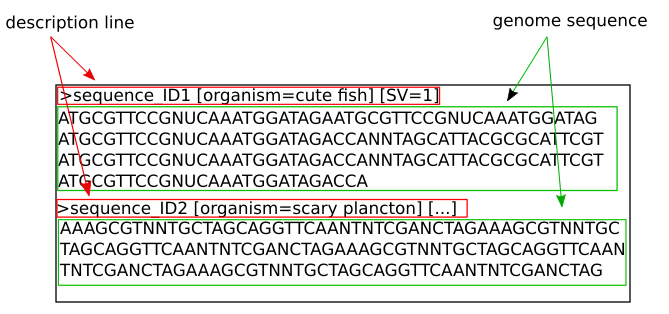
\includegraphics[scale = 0.5]{Figures/fastaex.png}
    \caption{Illustration of an example FASTA file }
    \label{fig:fasta}
\end{figure}

\paragraph{Short Reads}
On the other hand, the files containing the shorts reads to map to the reference genome are expected to be in \textsl{FASTQ} format \footnote{http://support.illumina.com/content/dam/illumina-support/help/BaseSpaceHelp_v2/Content/Vault/Informatics/Sequencing_Analysis/BS/swSEQ_mBS_FASTQFiles.htm}. The main difference between this format and the one presented below is that \textsl{FASTQ} allows the inclusion of the estimated quality score of the read for each symbol. For each read, one line corresponding to its ID, then the read symbols followed by a line containing only the symbol "+". Below this line are the quality scores, each position corresponding to their nucleoread counterpart. Hence, the global structure of a file following this format would be as represented in Figure \ref{fig:fastq}


\begin{figure}[H]
    \centering
    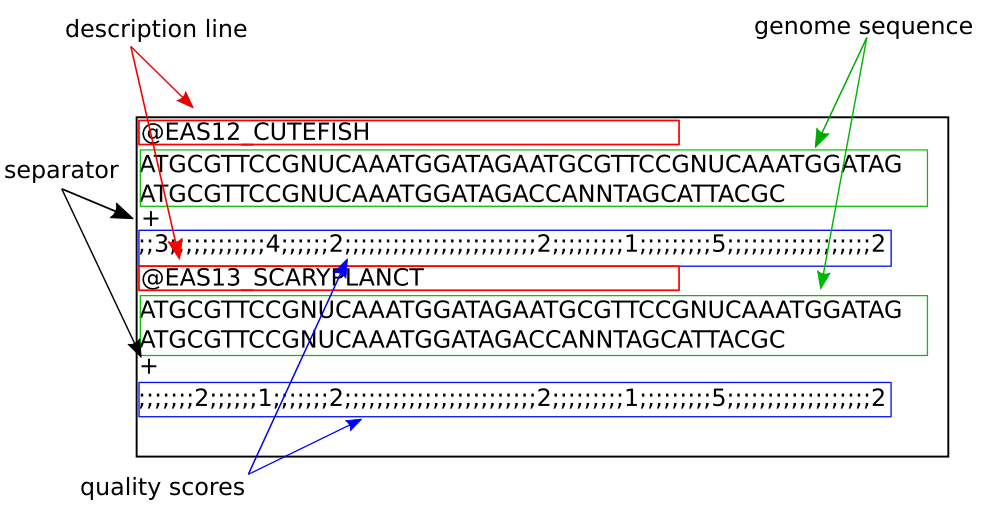
\includegraphics[scale = 0.35]{Figures/fastqex.png}
    \caption{Illustration of an example FASTQ file }
    \label{fig:fastq}
\end{figure}

\subsection{Output Files}

This program is also used to create files that will be used in the hardware implementation of the FM-Index. Those files are all the required structures, as showed in figure \ref{fig:fmindex}. Those files are described in the following paragraphs. 

\paragraph{Burrows-Wheeler Transform}

This file contains the whole BWT of an input reference sequence. The symbols are encoded as described in the previous section and it will be placed in the main memory of the hardware module.

\paragraph{Sampled FM-Index}

This file contains all the sampled "checkpoints" mentioned earlier in this document. All rows contain five 32-bit values, each of which corresponds to the number of occurences for each symbol at a given position in the BWT. Those checkpoints are taken every 128$^{th}$ symbols. This choice is based on the actual size of each checkpoints (5*32 bits), which is non-negligible and the fact that a simple scan of the \textit{BWT} from the current position to the nearest checkpoint is enough to determine the actual count value. Hence, providing constant time complexity with limited space cost.

\paragraph{Sampled Suffix Array}

This file contains samples of the suffix array, as mentioned in section 2.1.2.

\paragraph{Mapped Sequences}

Mapped sequences are returned in \textsl{SAM}  (Sequence Alignment/Map) format which provides a simple yet exhaustive description of each aligned read with respect to a reference text. Each rows contains 11 mandatory fields
, described in Figure \ref{fig:samf}, used to describe the alignment characteristics (e.g. name, reference name, quality, etc.) \\

\begin{figure}[H]
    \centering
    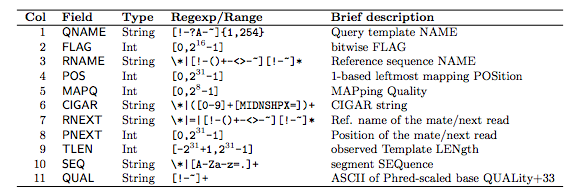
\includegraphics[scale = 0.78]{Figures/SAMv1_3.png}
    \caption{Mandatory fields of SAM format for each mapping}
    \label{fig:samf}
\end{figure}
\vspace*{4mm}

This format will allow a good result structure while keeping the formatting process rather simple and the amount of information to keep along the processing rather low. 

Figure \ref{fig:cpp_workflow} describes the program structure and execution flow along with the files it produces from the FM-Index structures :

\begin{figure}[H]
    \centering
    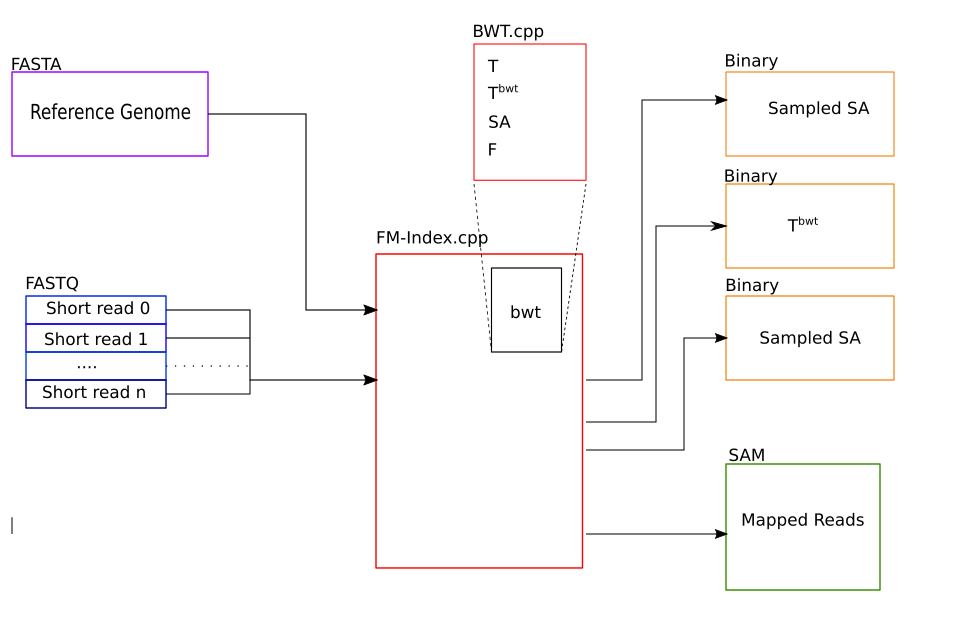
\includegraphics[scale = 0.4]{Figures/cpp_workflow.png}
    \caption{Illustration of the C++ software Execution}
    \label{fig:cpp_workflow}
\end{figure}



\section{Tests \& Results}

Using a Python reference \footnote{TODO cite https://github.com/egonelbre/fm-index}, it was possible to verify the output of the C++ software using a random DNA sequence. \\

The results showed that the program was behaving as expected ad provided correct references and mappings. \\

Sadly, the output format for the Mapped Reads, supposed to be in SAM, was not implemented.
